\documentclass[12pt]{beamer}
%\usepackage{beamerthemeHannover}
\usepackage{graphicx, clrscode, amsmath, amssymb, multicol}
\usepackage{verbatim}
\usetheme{Copenhagen} 

%\setbeamercolor{sidebar}{use=structure,bg=gray!20!green!60!white}
\setbeamertemplate{blocks}[rounded][shadow=true]


\title{Making Twitter Suck Less With Perl}
\author[Duke Leto]{Jonathan "Duke" Leto}

\date{}

\begin{document}
\frame{
    \frametitle{Making Twitter Suck Less With Perl}
    \framesubtitle{Speak Perl to your favorite $\mu$blogging service}
        \begin{center}
        
\includegraphics[width=3.00cm, height=1.50cm]{perl_republic}
        
\includegraphics[width=2.56cm, height=2.56cm]{twitter_logo}
        \end{center}
}

\frame{
    \frametitle{What sucks, but ain't Twitter's fault?}
    \begin{itemize}
    \item Following annoying people
    \item Having boring friends
    \item Twittershitters
    \end{itemize}
        \begin{center}
        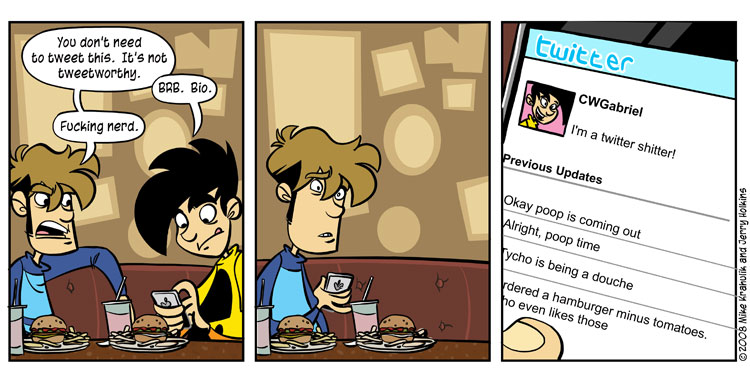
\includegraphics[width=6.00cm, height=3.50cm]{twittershitter}
        \end{center}
}

\frame{
    \frametitle{What \textcolor{red}{actually} sucks?}
    \begin{itemize}
    \item Interesting tweets buried in a sea of nonsense
    \item Tag spam (\#omg \#its \#hashtags \#allthewaydown)
    \item Skeezy webapps that steal your credentials
    \item Worms (StalkDaily)
    \item Marketing bots
    \item SEO crazies
    \end{itemize}

    Perl can help with most of these!
}

\begin{frame}
    \frametitle{How can Perl help?}
    \begin{itemize}
    \item Use the power of CPAN!
    \item Automate finding what you want
    \item Filter out what you don't care about
    \end{itemize}
\end{frame}

\begin{frame}[fragile]
    \frametitle{Net::Twitter}
    \begin{itemize}
    \item Uses Moose
    \item Works with Twitter and Identi.ca
    \item REST, Search and Twittervision API support
    \item OAuth and Basic Authentication
    \item 1 to 1 mapping with API
    \item Plenty of syntax sugar
    \item Net::Twitter::Lite
        \begin{itemize}
        \item Fewer Dependencies
        \item Same great taste
        \end{itemize}
    \end{itemize}
\end{frame}

\begin{frame}[fragile]
    \frametitle{Net::Twitter Basic Use}
    \begin{small}
    \begin{verbatim}
    my $nt  = Net::Twitter->new({
                 username => $user,
                 password => $pass,
                 traits   => [qw/API::REST/],
              });
    my $my_tl    = $nt->user_timeline({count=>5});
    my $buddy_tl = $nt->user_timeline({
                        screen_name => $buddy
                    });
    $nt->update('Perl rocks!');
    $nt->new_direct_message($buddy,$tweet);
    $nt->follow_new($cool_tweep);
    $nt->unfollow($seo_guy);

    \end{verbatim}
    \end{small}
\end{frame}

\begin{frame}[fragile]
    \frametitle{WWW::ItsABot}
    \textcolor{blue}{itsabot.com} has a constantly-updated database of Twitter bots.
    \begin{verbatim}
    use WWW::ItsABot qw/is_a_bot/;
    my $username = 'foobar';
    if ( is_a_bot($username) ) {
        print "$username is a bot\n";
    } else {
        print "$username is not a bot\n";
    }
    \end{verbatim}

    It ain't perfect, but it is pretty good. It may
    think some celebrities are bots and, really,
    it isn't that far off.

\end{frame}

\begin{frame}[fragile]
    \frametitle{Twitter::TagGrep}
    \textcolor{red}{grep} for Twitter timelines
    \begin{verbatim}
my $tg = Twitter::TagGrep->new( 
            prefix => '#!',
            tags => [ @tags ] 
        );
my $timeline = $twit->friends_timeline({count=>200});
my @matches  = $tg->grep_tags($timeline);
for my $tweet (@matches) {
    print join(', ', @{$tweet->{tags}}), ": ",
                $tweet->{text},"\n";
}
    \end{verbatim}
\end{frame}

%\begin{frame}[fragile]
%    \frametitle{TEMP}
%    \begin{verbatim}
%    \end{verbatim}
%\end{frame}

\begin{frame}[fragile]
    \frametitle{Log::Dispatch::Twitter}
    Add a Twitter user as a Log::Dispatch logger easily!
    \begin{verbatim}
    use Log::Dispatch;
    use Log::Dispatch::Twitter;
    my $logger = Log::Dispatch->new;
    $logger->add(Log::Dispatch::Twitter->new(
        username  => $username,
        password  => $password,
        min_level => "error",
        name      => "twitter",
    ));
    \end{verbatim}
\end{frame}

\begin{frame}[fragile]
    \frametitle{Task::Twitter}
Get the modules mentioned in this talk easily:
    \begin{verbatim}
    sudo cpan Task::Twitter
    \end{verbatim}
Hitting a CPAN mirror near you soon!
\end{frame}

\begin{frame}
    \frametitle{What I'm working on}
    \begin{itemize}
    \item Visualizing Twitter connections with GraphViz
        \begin{itemize}
        \item Colorized based on user characteristics
        \end{itemize}
    \item Extendable Twitter Bot framework
    \item Follow me at github.com/leto or @dukeleto on Twitter
    \end{itemize}
    What are \textcolor{red}{you} working on?

\end{frame}

\begin{frame}[fragile]
    \frametitle{Conclusions}
    \begin{itemize}
    \item Most of the annoying things about Twitter can be solved with a few lines of Perl.
    \item There is an amazing amount of data waiting to be tapped.
    \item Perl to the rescue!
    \end{itemize}

\end{frame}

\begin{frame}[fragile]
    \frametitle{Thanks!}
    \begin{itemize}
    \item Open Source Bridge volunteers
    \item Larry
    \item Marc Mims for Net::Twitter
    \item The Twitter Dev Team
    \item All my fellow Open Source Citizens
    \end{itemize}
\end{frame}
\end{document}
